\chapter{Analysis of high-temperature events}

\label{Chapter5}

In this chapter, the products of HTE monitoring from MITIP will presented firstly using scenes worldwide which contains volcanoes, large scale lava flow and wild fires. In section 5.2, the HTE monitoring results of MITIP will be compared with the results of the Zhukov's algorithm, which is used to process the TET-1 imagery originally.\\
%----------------------------------------------------------------------------------------
%	SECTION 1
%----------------------------------------------------------------------------------------

\section{High-temperature events}
In this section, the HTE monitoring results are presented. For the process of all scenes, the maps of MODIS water vapor, ASTER DEM and 8.6 $\mu$m emissivity maps were provided and resampled to the TET-1 imagery's size and pixel size. The input TET-1 MIR and TIR TOA radiance imageries are scaled with scale factor 1.15 and 1.05 respectively.\\

%-----------------------------------
%	SUBSECTION 1
%-----------------------------------

\subsection{Volcanoes}
First of all, the HTE monitoring products of Etna and Stromboli in the date 2016.06.22 are presented. Both of them only occupy a little spaces in images because of their small sizes.\\

\begin{figure}[!htbp]
\centering
\subfigure[MIR band]{
\label{fig:Etna_mir_tem}
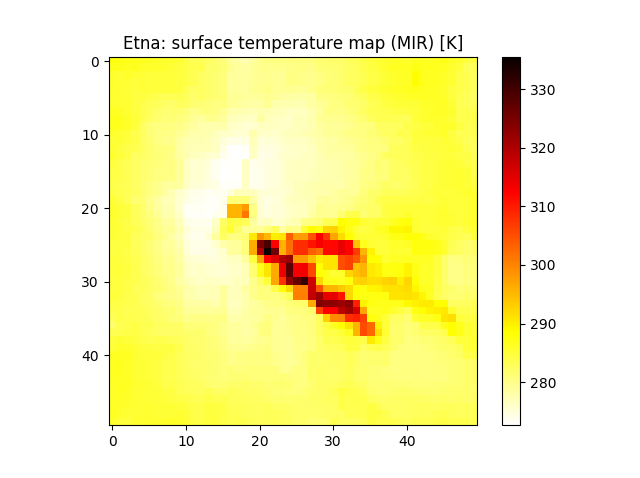
\includegraphics[width = 0.8\linewidth]{temp_map_etna_mir.png}}
\hspace{0.1in}
\subfigure[TIR band]{
\label{fig:Etna_tir_tem}
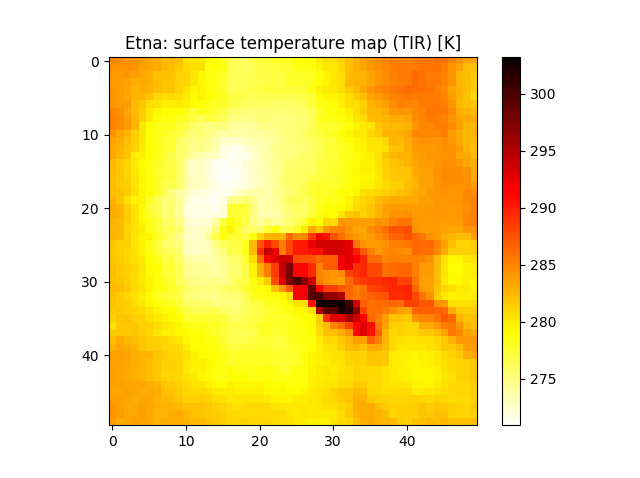
\includegraphics[width = 0.8\linewidth]{temp_map_etna_tir.png}}
\caption{Surface temperature maps of Etna 2014.06.22.}
\label{fig:Etna_sur_tem}
\end{figure}

\noindent As Figure \ref{fig:Etna_sur_tem} shows, the surface temperatures of the lava are around 310 K to 340K in MIR band and 290K to 310K in TIR band. The effective target temperature in sub-pixel resolution and effective target pixel fraction as well as the FRP are shown in Figure \ref{fig:Etna_HTE} and Figure \ref{fig:Etna_frp}. We can see that not all hot pixels in the surface temperature maps are solved for the effective target temperature and target pixel fraction due to numerical reasons. The hottest areas of the Etna are around 850 K. It can be notice that the higher the effective target temperature in one pixel, the lower the effective target pixel fraction of it. Because the pixel temperature and background temperature are pre-determined.\\

\begin{figure}[!htbp]
\centering
\subfigure[Effective target temperature]{
\label{fig:Etna_eff_tem}
\includegraphics[width = 0.8\linewidth]{Effective_target_tem_etna.png}}
\hspace{0.1in}
\subfigure[Effective target pixel fraction]{
\label{fig:Etna_eff_fra}
\includegraphics[width = 0.8\linewidth]{Effective_target_pixel_frac_etna.png}}
\caption{HTE monitoring products of Etna 2014.06.22.}
\label{fig:Etna_HTE}
\end{figure}

\begin{figure}[!htbp]
\centering
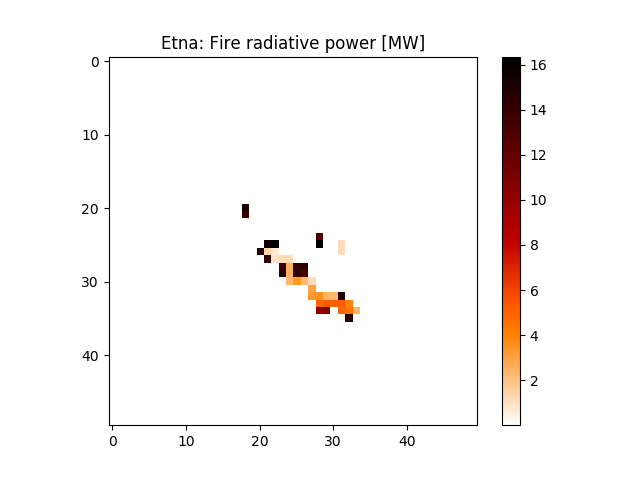
\includegraphics[width=0.8\linewidth]{frp_etna.png}
\caption{FRP of Etna 2014.06.22.}
\label{fig:Etna_frp}
\end{figure}

\noindent Stromboli island is one of the Aeolian island of Italy. The Stromboli volcano is one of the most active volcanoes on Earth. It has been nearly continuous erupting for about 2000 years. Since there is a small town in Stromboli island, the prediction and monitoring of the eruption of the Stromboli volcano is of great importance. The figure \ref{fig:Strom_sur_tem} shows the surface temperature maps of Stromboli in MIR and TIR band respectively of the date 2014.06.22. It can be noticed that in evening, the temperature of the sea surface is higher than the temperature of the land surface.\\

\begin{figure}
\centering
\subfigure[MIR band]{
\label{fig:Strom_mir_tem}
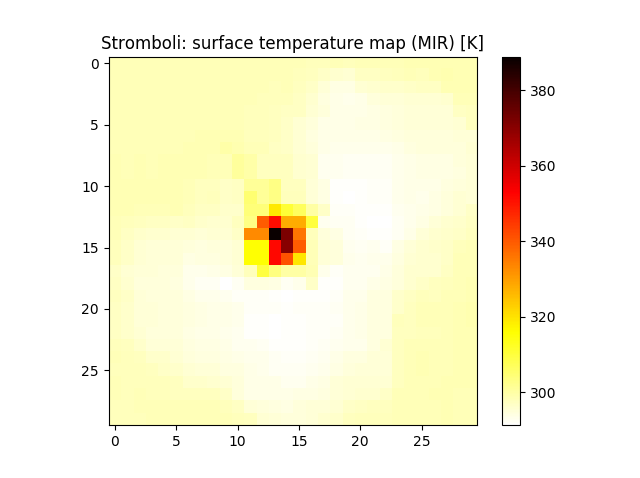
\includegraphics[width = 0.8\linewidth]{strom_tem_mir.png}}
\hspace{0.1in}
\subfigure[TIR band]{
\label{fig:Strom_tir_tem}
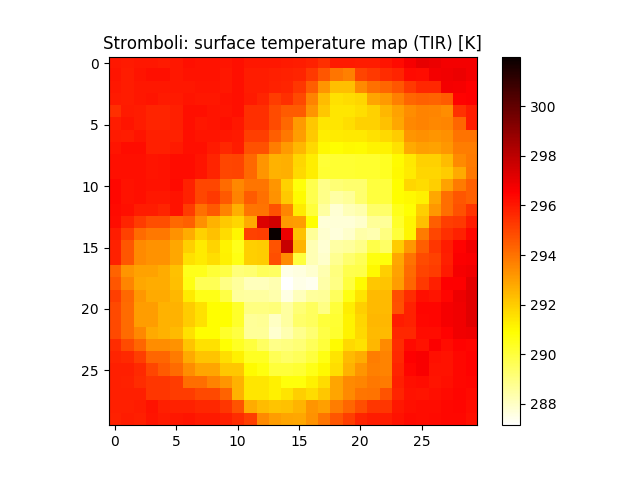
\includegraphics[width = 0.8\linewidth]{strom_tem_tir.png}}
\caption{Surface temperature maps of Stromboli 2014.06.22.}
\label{fig:Strom_sur_tem}
\end{figure}

\noindent The effective target temperature and effective target pixel fraction of Stromboli in date 2014.06.22 are shown in Figure \ref{fig:Strom_HTE} and the fire radiative power in Figure \ref{fig:Strom_frp}. We can see that the hottest areas of the Stromboli is above 1400 K which only occupy a small fraction of the pixels as well.\\

\begin{figure}[!htbp]
\centering
\subfigure[Effective target temperature]{
\label{fig:Strom_eff_tem}
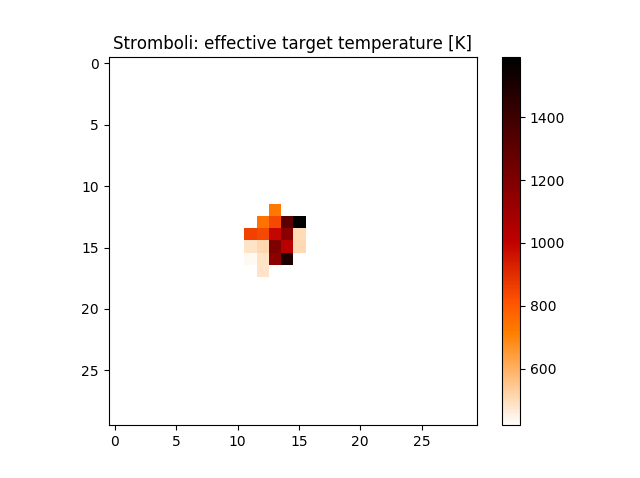
\includegraphics[width = 0.8\linewidth]{strom_eff_tem_strom.png}}
\hspace{0.1in}
\subfigure[Effective target pixel fraction]{
\label{fig:Strom_eff_fra}
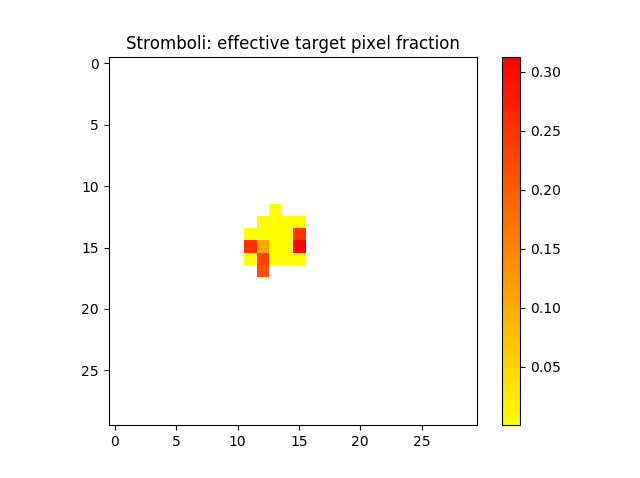
\includegraphics[width = 0.8\linewidth]{strom_eff_pixel_frac_strom.png}}
\caption{HTE monitoring products of Stromboli 2014.06.22.}
\label{fig:Strom_HTE}
\end{figure}

\begin{figure}[!htbp]
\centering
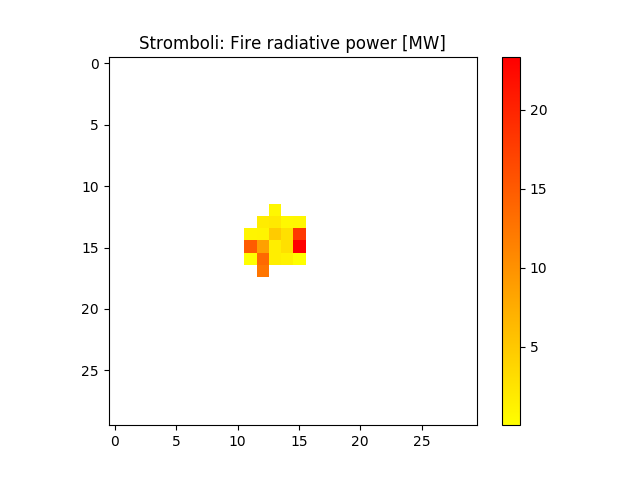
\includegraphics[width=0.8\linewidth]{frp_strom.png}
\caption{FRP of Stromboli 2014.06.22.}
\label{fig:Strom_frp}
\end{figure}

\noindent Etna and Stromboli are both small volcanoes which occupy only a few pixels in the imageries. In contrast, the eruption of Bardarbunga is much more intensive and its lava occupies a much larger area. Bardarbunga is a subglacial stratovolcano located in Iceland. The last eruption of Bardarbunga is from August 2014 to February 2015. Figure \ref{fig:Bar_sur_tem} presents the surface temperature map of Bardarbunga in date 2014.09.14.\\

\begin{figure}
\centering
\subfigure[MIR band]{
\label{fig:Bar_mir_tem}
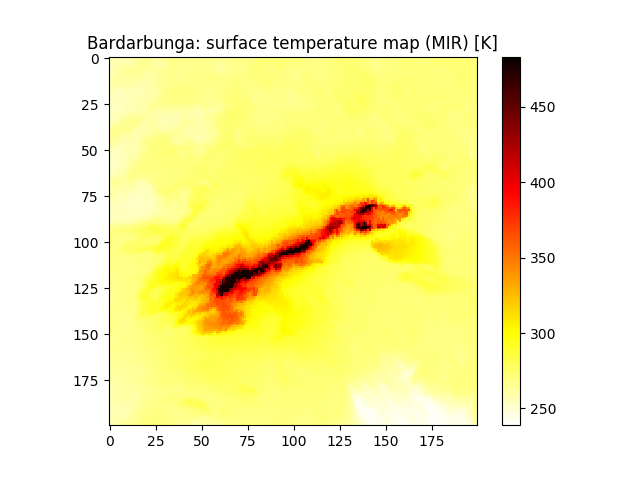
\includegraphics[width = 0.8\linewidth]{Bar_tem_mir.png}}
\hspace{0.1in}
\subfigure[TIR band]{
\label{fig:Bar_tir_tem}
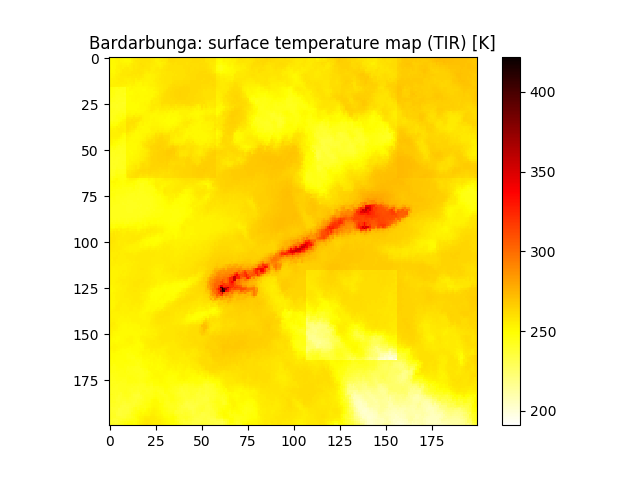
\includegraphics[width = 0.8\linewidth]{Bar_tem_tir.png}}
\caption{Surface temperature maps of Bardarbunga 2014.09.14.}
\label{fig:Bar_sur_tem}
\end{figure}

\noindent It is clear that the erupted lava occupied a large area and the temperature of it is between 400 K and 500 K in MIR band and 350 K to 450 K in TIR band. Figure \ref{fig:Bar_HTE} and Figure \ref{fig:Bar_frp} give the effective target temperature and effective target pixel fraction as well as FRP maps.\\

\begin{figure}[!htbp]
\centering
\subfigure[Effective target temperature]{
\label{fig:Bar_eff_tem}
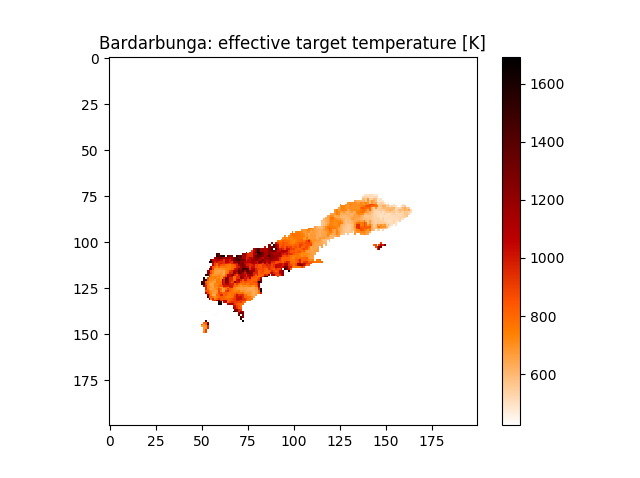
\includegraphics[width = 0.8\linewidth]{Bar_eff_tem.png}}
\hspace{0.1in}
\subfigure[Effective target pixel fraction]{
\label{fig:Bar_eff_fra}
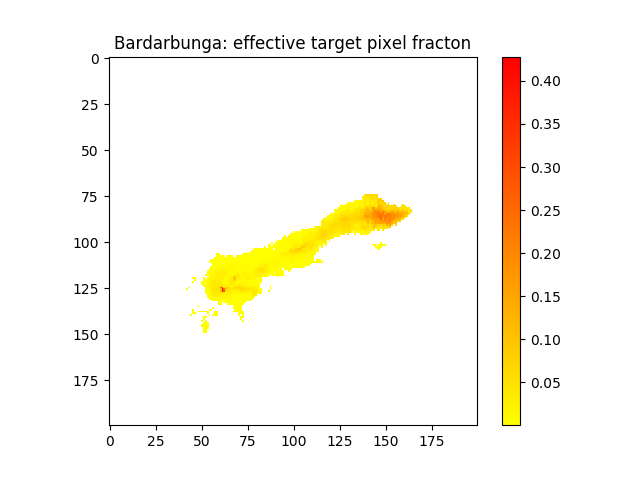
\includegraphics[width = 0.8\linewidth]{Bar_eff_pixel_frac.png}}
\caption{HTE monitoring products of Bardarbunga 2014.09.14.}
\label{fig:Bar_HTE}
\end{figure}

\begin{figure}[!htbp]
\centering
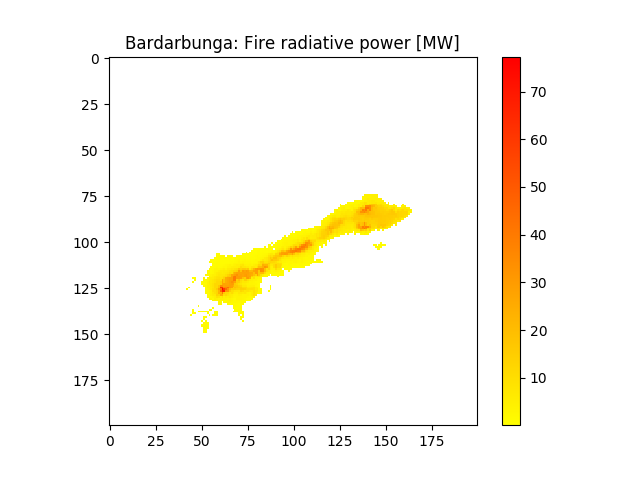
\includegraphics[width=0.8\linewidth]{Bar_frp.png}
\caption{FRP of Bardarbunga 2014.09.14.}
\label{fig:Bar_frp}
\end{figure}
%-----------------------------------
%	SUBSECTION 2
%-----------------------------------

\subsection{Fire events}
Besides volcanoes, wild fires are another kind of high-temperature events need to be paid attention to. Here, the HTE monitoring results of Portugal wild fires is presented. Figure \ref{fig:Por_sur_tem} shows the surface temperature maps in MIR and TIR band. The fire edges can be seen clearly in the surface temperature maps.\\

\begin{figure}
\centering
\subfigure[MIR band]{
\label{fig:Por_mir_tem}
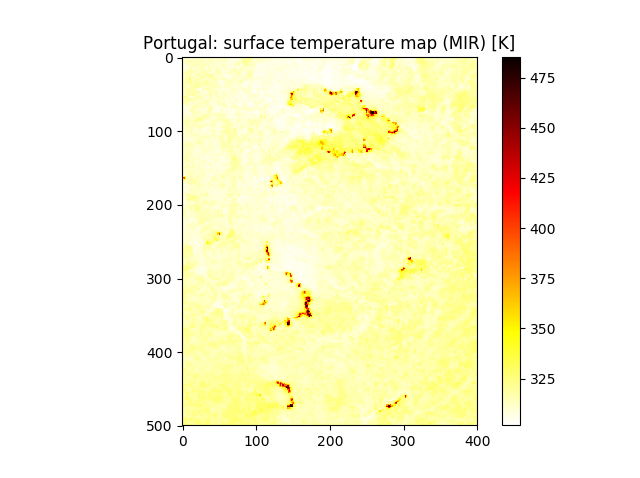
\includegraphics[width = 0.8\linewidth]{Por_tem_mir.png}}
\hspace{0.1in}
\subfigure[TIR band]{
\label{fig:Por_tir_tem}
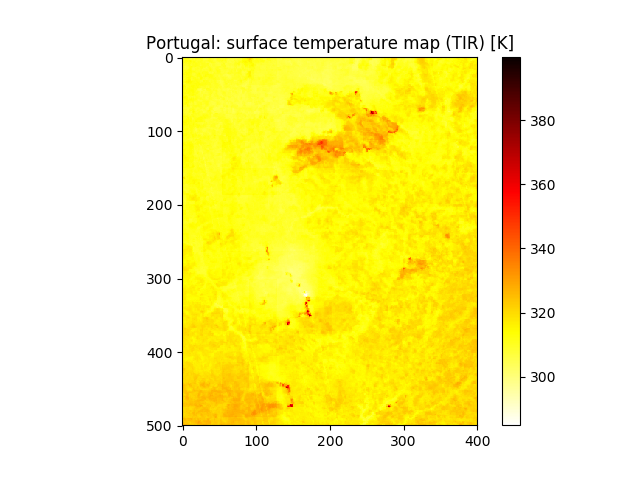
\includegraphics[width = 0.8\linewidth]{Por_tem_tir.png}}
\caption{Surface temperature maps of Portugal wild fires in 2016.08.11.}
\label{fig:Por_sur_tem}
\end{figure}

\noindent Figure \ref{fig:Por_HTE} and Figure \ref{fig:Por_frp} are the effective target temperature and effective target pixel fraction as well as fire radiative power maps. We can see the large scale and the scorching temperatures of the wild fires.

\begin{figure}[!htbp]
\centering
\subfigure[Effective target temperature]{
\label{fig:Por_eff_tem}
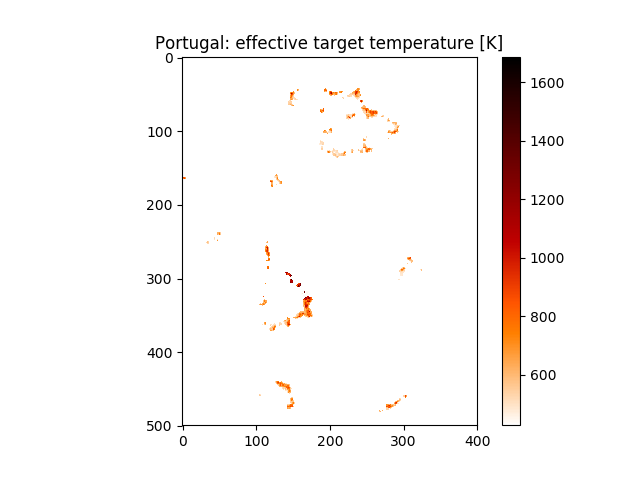
\includegraphics[width = 0.8\linewidth]{Por_eff_tem.png}}
\hspace{0.1in}
\subfigure[Effective target pixel fraction]{
\label{fig:Por_eff_fra}
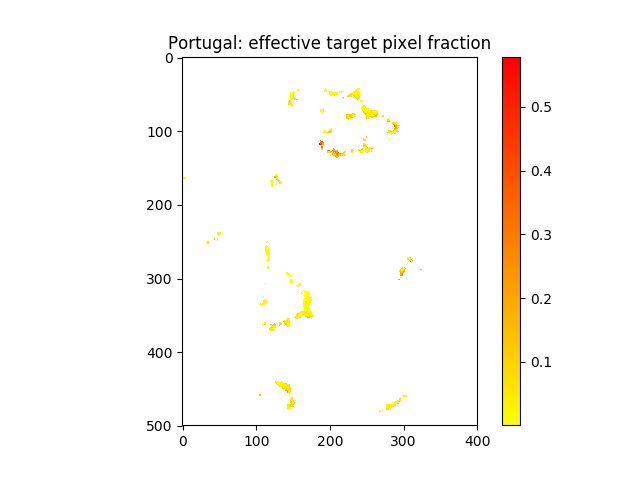
\includegraphics[width = 0.8\linewidth]{Por_eff_pixel_frac.png}}
\caption{HTE monitoring products of Portugal wild fires in 2016.08.11.}
\label{fig:Por_HTE}
\end{figure}

\begin{figure}[!htbp]
\centering
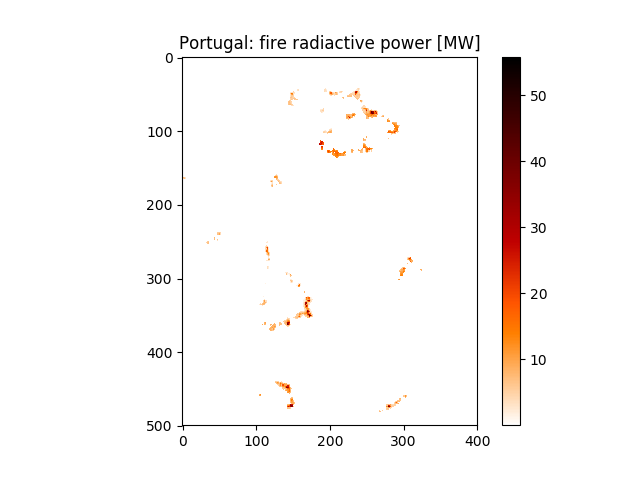
\includegraphics[width=0.8\linewidth]{Por_frp.png}
\caption{FRP of Portugal wild fires in 2016.08.11.}
\label{fig:Por_frp}
\end{figure}

%----------------------------------------------------------------------------------------
%	SECTION 2
%----------------------------------------------------------------------------------------

\section{Comparison with the results of the Zhukov's algorithm}
In this section, the HTE monitoring products of MITIP are compared with the results of Zhukov's algorithm, which used to process the TET-1 imagery originally.\\

%-----------------------------------
%	SUBSECTION 1
%-----------------------------------

\subsection{Brief description of Zhukov's algorithm}
Unlike other hot spot detection algorithms, the Zhukov's algorithm carries out a bundle of tests to filter out clouds, warm surfaces and sun glints etc first and then performs fire pixel detection. It uses the dual channel method stated in Chapter 2 to determine effective fire temperature in sub-pixel resolution as well. However, the Zhukov's algorithm detects and quantifies the hot area by means of per cluster instead of per pixel as MITIP method dose. After the detection of hot spots, the Zhukov's algorithm aggregates hot pixels which are adjacent to each other to form a hot cluster and the temperature of this cluster and its area etc are estimated.\\

\begin{figure}[!htbp]
\centering
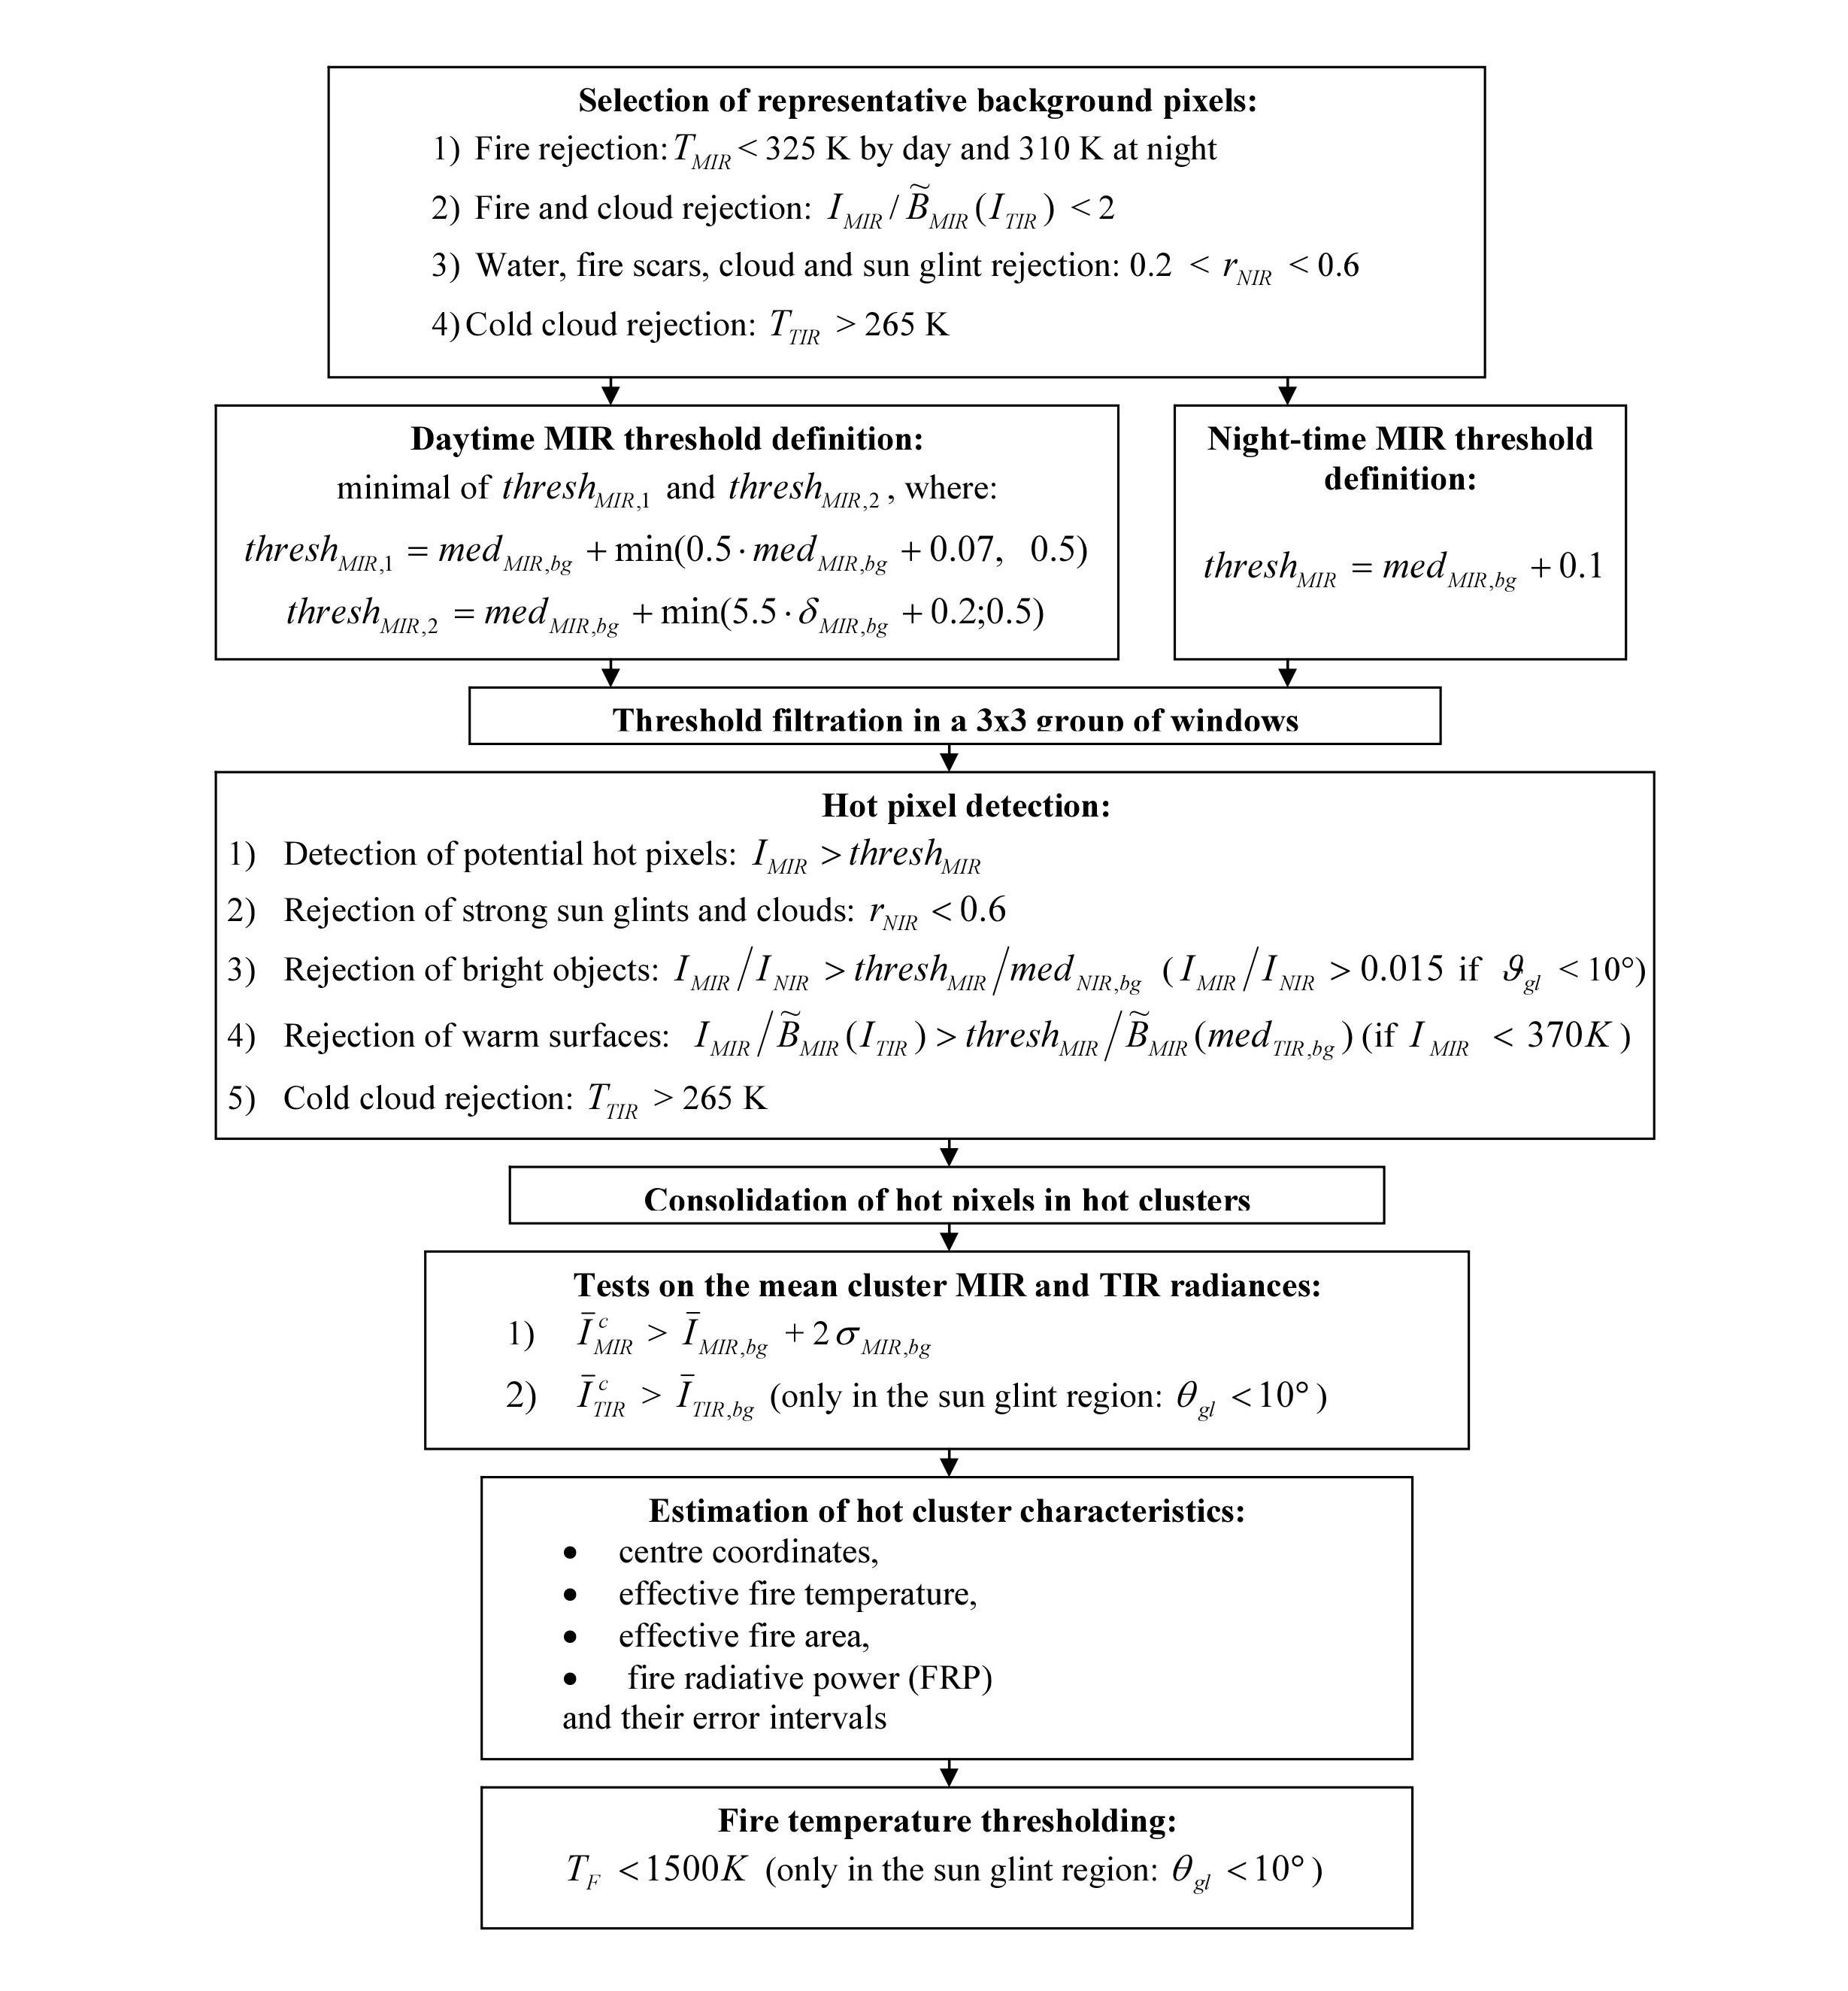
\includegraphics[width=0.8\linewidth]{Zhukov_algorithm.jpg}
\caption{Flow chart of the Zhukov's algorithm.}
\label{fig:Zhu_alg}
\end{figure}

\noindent The brief procedure of Zhukov's algorithm is shown in Figure \ref{fig:Zhu_alg}.\\

%-----------------------------------
%	SUBSECTION 2
%-----------------------------------

\subsection{From pixel-based to cluster-based analysis}
In contrast to Zhukov's algorithm, the MITIP method performs a pixel-based analysis. Consequently, in order to compare the results of the MITIP method and Zhukov's algorithm, a procedure is developed to shift the MITIP's original pixel-based results to a cluster-based results because it is much more difficult to derive each pixel's temperature from the characteristics of the whole cluster. \\

\noindent The procedure is described as follows. The input is the effective target pixel fraction map and effective target temperature map which is converted to a vector file afterwards. The connected pixels will then form a polygon feature with which a cluster will come into being. Then every polygon feature in the vector file is extracted and converted to a raster file acts as a mask file. The mask file is used to extract AOI in the effective target temperature map and zonal statistics is carried out over the AOI. The final output is the cluster's temperature and size. The cluster's temperature is the weighted average of the effective target temperatures of pixels within this cluster and the weights are the corresponding effect target pixel fractions. The size of the cluster is denoted by the number of pixels. The Figure \ref{fig:P2C} shows the flow chart of the described procedure.\\

\begin{figure}[!htbp]
\centering
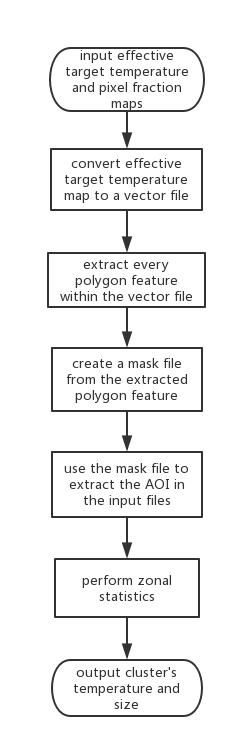
\includegraphics[width=0.4\linewidth]{Procedure.png}
\caption{Flow chart of the pixel-based result to the cluster-based result.}
\label{fig:P2C}
\end{figure}

%-----------------------------------
%	SUBSECTION 3
%-----------------------------------

\subsection{Comparison}
After converting MITIP's pixel-based results to cluster-based results, the comparison between MITIP and Zhukov's algorithm are able to carry out. Similar with what has be done in previous section, the comparison is done over small volcanoes, large scale lava and wild fires.\\

\noindent Firstly, the scenes of Etna in date 2014.07.21 has been processed by these two method and shown in Figure \ref{fig:Etna_comp}. Blue line is the boundary of the cluster detected by Zhukov's algorithm. Green line is the boundary of the cluster produced by MITIP. First of all, due to the reason of resampling, there are some shifts between the locations of detected cluster of MITIP and Zhukov's algorithm. Second, because the MITIP is a pixel-based method, due to the numerical reasons, some pixels will fail during the determination of effective target temperatures. This is the reason why inside the cluster derived from MITIP surface temperature map, there are several missing pixels. Besides these two points, we can see that the location of these two clusters are almost overlapped and the size of them are almost identical as well.\\

\begin{figure}[!htbp]
\centering
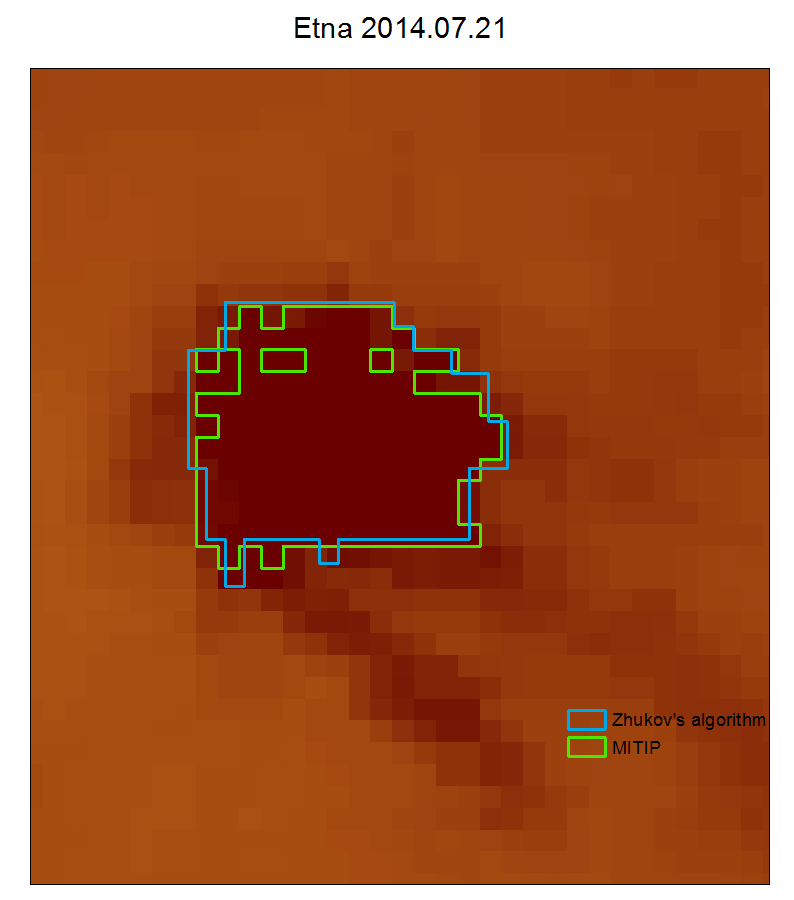
\includegraphics[width=0.8\linewidth]{Etna_20140721.png}
\caption{Etna 2014.07.21. The background picture is the surface temperature map in MIR band from MITIP. Blue line is the boundary of the cluster detected by Zhukov's algorithm. Green line is the boundary of the cluster produced by MITIP.}
\label{fig:Etna_comp}
\end{figure}

\begin{table}[!ht]
\caption{Etna 2014.07.21. Comparison between MITIP and Zhukov's algorithm.}
\centering
\begin{tabular}{c|c|c|c|c}
\hline\hline
\textbf{Method} & \multicolumn{3}{|c|}{\textbf{Temperature [K]} }& \textbf{Cluster size} \\
\hline
\multirow{2} * {Zhukov} & min &mean & max & \multirow{2}*{127} \\ \cline{2 - 4}
 & 611 & 633.5 & 661.3 &  \\
 \hline
 MITIP & \multicolumn{3}{|c|}{644.3} & 123 \\
 \hline\hline
\end{tabular}
\label{Etna_comp}
\end{table}

\noindent From Table \ref{Etna_comp}, it can be seen that besides the mean temperature of the cluster, Zhukov's algorithm also provides minimal and maximal temperatures. The cluster's temperature derived by MITIP is within the minimal and maximal temperature range and differs with the mean temperature around 11 K. The cluster size differs with 4 pixels. All of these enable us to say that the results of HTE monitoring of Zhukov's algorithm and MITIP using Etna scenes in date 2014.07.21 are in accord with each other very well.\\

\noindent Figure \ref{fig:Strom_comp} shows the comparison results using the Stromboli scene in date 2014.07.03. Blue line is the boundary of the cluster detected by Zhukov's algorithm. Green line is the boundary of the cluster produced by MITIP. As states before, there is a bit shift between them and the cluster detected by Zhukov's algorithm are a bit smaller than the cluster derived from MITIP, which is also presented in Table \ref{Strom_comp}. Again, the two results agree with each other as well.\\

\begin{figure}[!htbp]
\centering
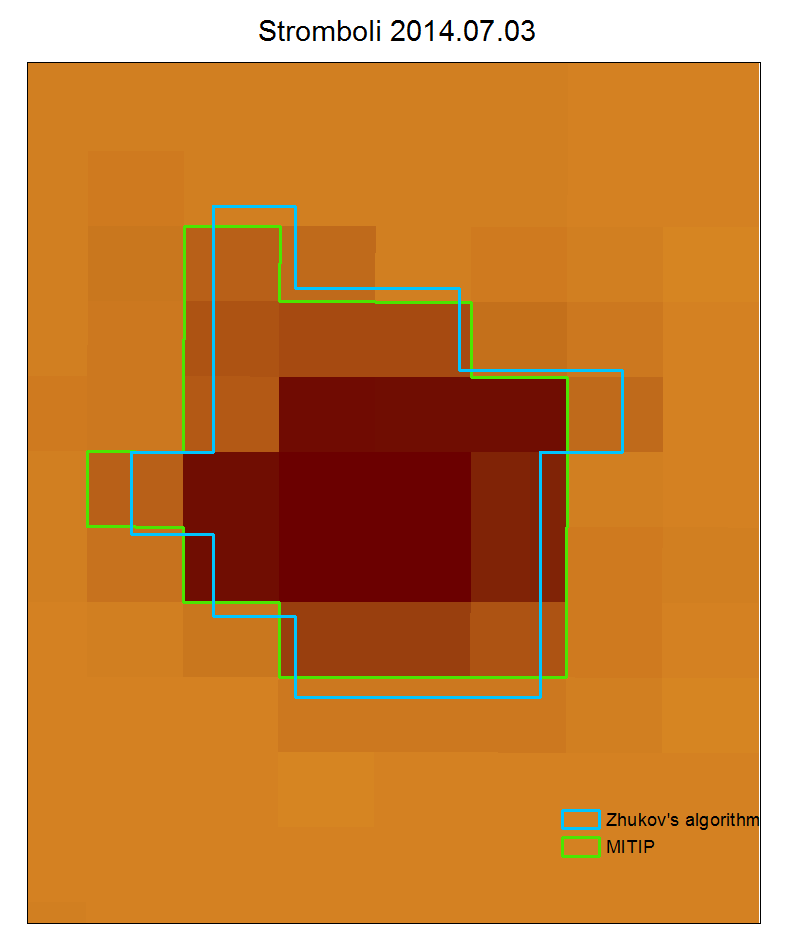
\includegraphics[width=0.8\linewidth]{stromboli_20140703.png}
\caption{Stromboli 2014.07.03. The background picture is the surface temperature map in MIR band from MITIP. Blue line is the boundary of the cluster detected by Zhukov's algorithm. Green line is the boundary of the cluster produced by MITIP.}
\label{fig:Strom_comp}
\end{figure}

\begin{table}[!ht]
\caption{Stromboli 2014.07.03. Comparison between MITIP and Zhukov's algorithm.}
\centering
\begin{tabular}{c|c|c|c|c}
\hline\hline
\textbf{Method} & \multicolumn{3}{|c|}{\textbf{Temperature [K]} }& \textbf{Cluster size} \\
\hline
\multirow{2} * {Zhukov} & min &mean & max & \multirow{2}*{16} \\ \cline{2 - 4}
 & 504.6 & 529.9 & 564.9 &  \\
 \hline
 MITIP & \multicolumn{3}{|c|}{521.0} & 20 \\
 \hline\hline
\end{tabular}
\label{Strom_comp}
\end{table}

\noindent The Etna and Stromboli both occupy a few numbers of pixels merely in the imageries. Following is the comparison results using scene of Bardarbunga in date 2014.09.14, in which the hot area occupies a large area as shown in Figure \ref{fig:Bar_comp}. It can be noticed that the detected cluster by Zhukov's algorithm, which includes a lot of additional no-hot pixels, is much larger than the cluster derived by MITIP, which describes the boundary of the cluster much precisely as shown in Figure \ref{fig:Bar_comp}.\\

\begin{figure}[!htbp]
\centering
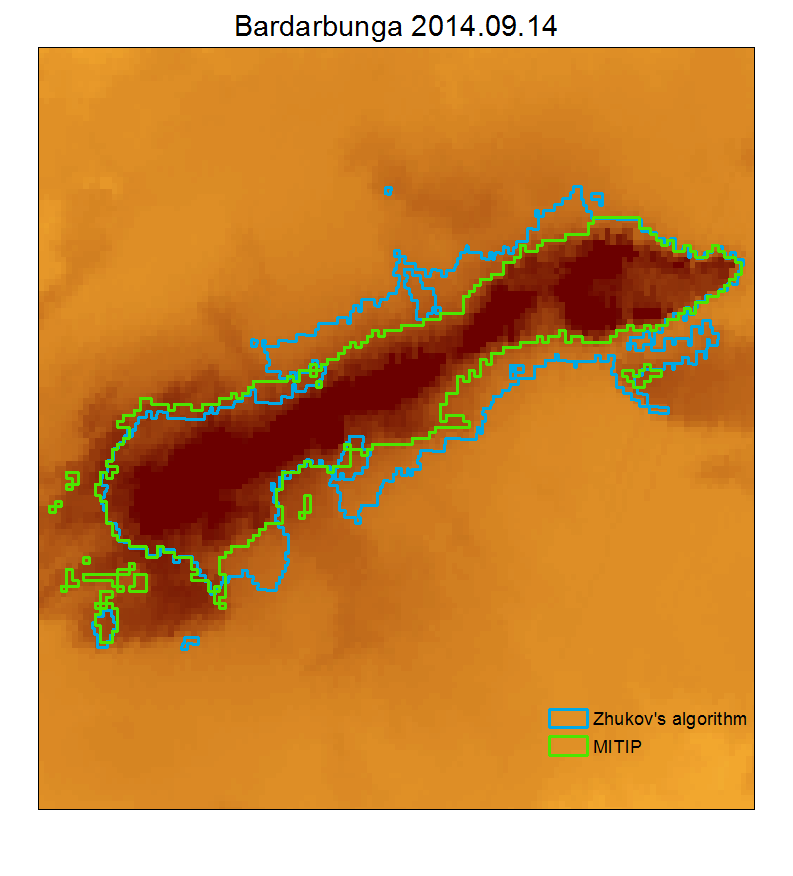
\includegraphics[width=0.8\linewidth]{Bardarbunga_20140914.png}
\caption{Bardarbunga 2014.09.14. The background picture is the surface temperature map in MIR band from MITIP. Blue line is the boundary of the cluster detected by Zhukov's algorithm. Green line is the boundary of the cluster produced by MITIP.}
\label{fig:Bar_comp}
\end{figure}

\begin{table}[!ht]
\caption{Bardarbunga 2014.09.14.. Comparison between MITIP and Zhukov's algorithm.}
\centering
\begin{tabular}{c|c|c|c|c}
\hline\hline
\textbf{Method} & \multicolumn{3}{|c|}{\textbf{Temperature [K]} }& \textbf{Cluster size} \\
\hline
\multirow{2} * {Zhukov} & min &mean & max & \multirow{2}*{2461} \\ \cline{2 - 4}
 & 646.0 & 653.8 & 652.0 &  \\
 \hline
 MITIP & \multicolumn{3}{|c|}{661.3} & 2025 \\
 \hline\hline
\end{tabular}
\label{Bar_comp}
\end{table}

\noindent From Table \ref{Bar_comp} we can see that the cluster's temperature derived from MITIP exceeds the max temperature given by Zhukov's algorithm because the result of MITIP is concentrated in the hottest area while the cluster detected by Zhukov's algorithm includes too many normal-temperature pixels which resulted in the decrement of the cluster's temperature. The cluster size provided by Zhukov's algorithm is also much larger than the cluster size given by MITIP with around 450 pixels.\\

\noindent The HTE monitoring results about the wild fires are also compared. Figure \ref{fig:Chile_comp} shows the comparison result using the scene of Chile wild fires. The wild fires cover a large amount of areas and divide into several parts. Three large areas \emph{a}, \emph{b} and \emph{c1}, \emph{c2}  will be used in comparison which denoted in the Figure \ref{fig:Chile_comp} as well.

\begin{figure}[!htbp]
\centering
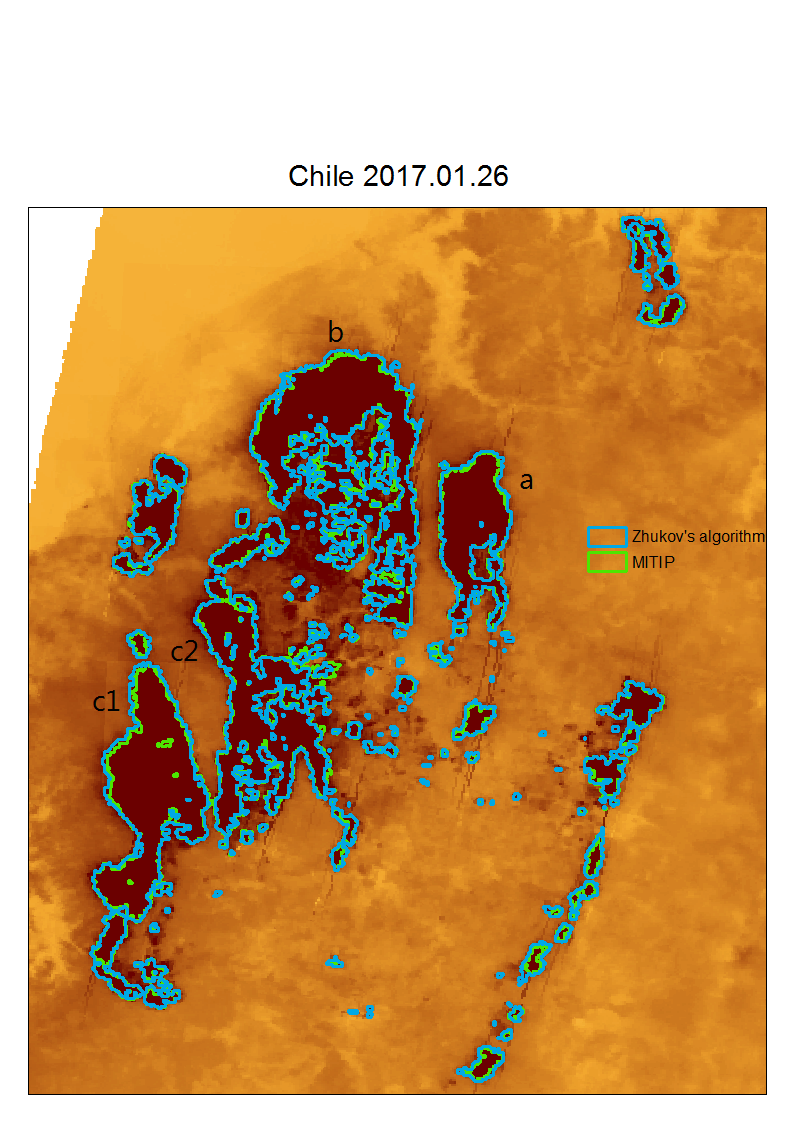
\includegraphics[width=0.8\linewidth]{Chile_20160126_note.png}
\caption{Chile 2016.01.26. The background picture is the surface temperature map in MIR band from MITIP. Blue line is the boundary of the cluster detected by Zhukov's algorithm. Green line is the boundary of the cluster produced by MITIP.}
\label{fig:Chile_comp}
\end{figure}

\begin{table}[!ht]
\caption{Chile 2016.01.26. Comparison between MITIP and Zhukov's algorithm.}
\centering
\begin{tabular}{c|c|c|c|c|c}
\hline\hline
\textbf{Loc.} & \textbf{Method} & \multicolumn{3}{|c|}{\textbf{Temperature [K]}} & \textbf{Cluster size} \\
\hline
\multirow{3}*{a} & \multirow{2}*{Zhukov} & min & mean & max & \multirow{2} * {1804} \\ \cline{3 - 5}
 & & 635.3 & 641.4 & 648.1 & \\ \cline{2 - 6}
 & MITIP & \multicolumn{3}{|c|}{656.7} & 2046 \\ 
\hline
\multirow{3}*{b} & \multirow{2}*{Zhukov} & min & mean & max & \multirow{2} * {3846} \\ \cline{3 - 5}
 & & 617.6 & 626.9 & 637.0 & \\ \cline{2 - 6}
 & MITIP & \multicolumn{3}{|c|}{602.0} & 4500 \\ 
\hline
\multirow{4}*{c} & \multirow{3}*{Zhukov} & min & mean & max & \\ \cline{3 - 6}
 & &c1:  612.0 & 615.2 & 618.5 & 3863 \\ \cline{3 - 6}
 & &c2:  612.9 & 619.9 & 627.5 & 3185 \\ \cline{2 - 6}
 & MITIP & \multicolumn{3}{|c|}{625.0} & 7829 \\ 
\hline\hline
\end{tabular}
\label{Bar_comp}
\end{table}

\noindent As Table \ref{Bar_comp} shows, the cluster's temperature derived from MITIP differs with the mean temperature given by Zhukov's algorithm at most 24 K which is the case of area \emph{b}. Area \emph{c} shows the largest differences of the results between the MITIP and Zhukov's algorithm. The Zhukov's algorithm take the area \emph{c1} and \emph{c2} as two different hot clusters. But as shown in Figure \ref{fig:Chile_comp2}, these two hot areas are connected by one single pixel in the HTE monitoring result of MITIP, which merges these two hot areas into one hot cluster.\\

\begin{figure}[!htbp]
\centering
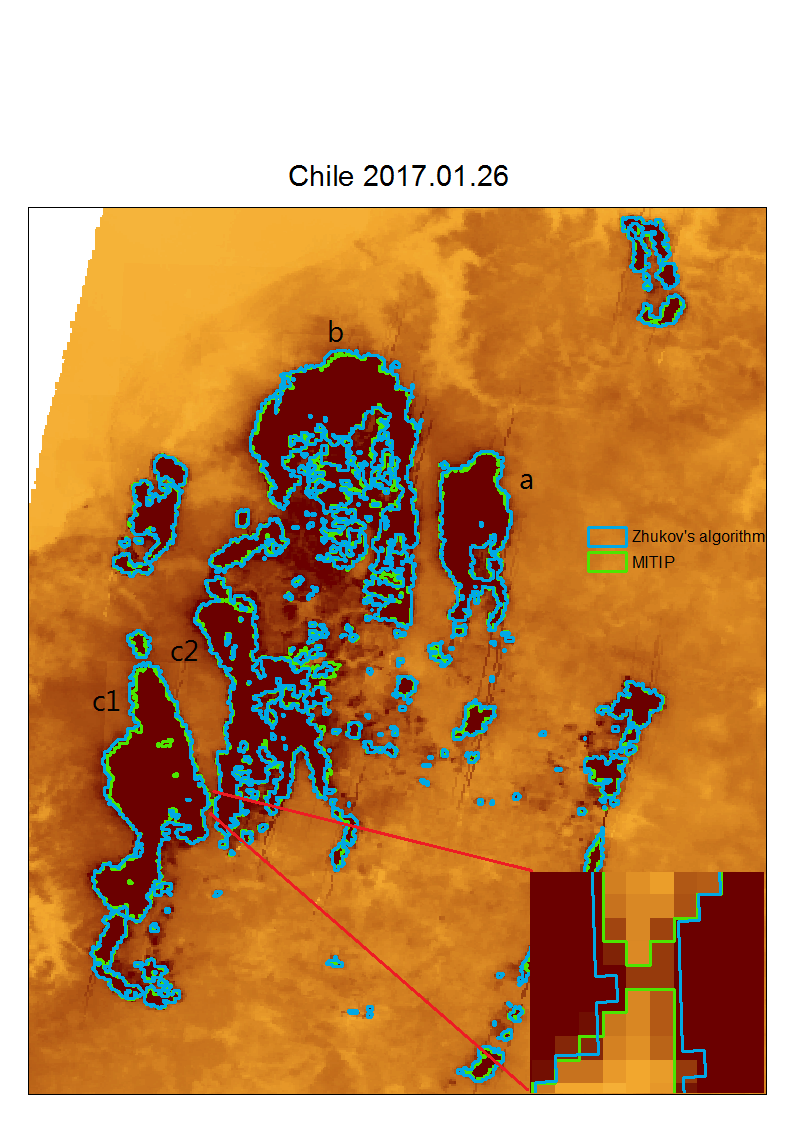
\includegraphics[width=0.8\linewidth]{Chile_20160126_note2.png}
\caption{Chile 2016.01.26. Sub-figure in the lower right corner shows that the two hot areas \emph{c1} and \emph{c2} are connected by one pixel in the result of MITIP method which merges these two hot areas into one hot cluster.}
\label{fig:Chile_comp2}
\end{figure}